\section{Usage Scenarios}
\subsection{Experimentation}
\subsubsection{Creation of Non-Realtime Multiplex}
The creation of a ETI file containing two programmes, one DAB and one
\dabplus{} is covered in section \ref{sec-files}.

\subsubsection{Modulation of ETI for Offline Processing}
The ETI file generated before can then be used with ODR-DabMod to generate a
file containing I/Q samples. Here, we must chose between using the command line
or the configuration file. For a very simple example, using the command line
makes sense, but for more advanced features it is preferable to use a
configuration file. For illustration, we will present both.

To modulate the file \texttt{myfirst.eti} into \texttt{myfirst.iq}, with the
default options, the command is simply

\begin{lstlisting}
odr-dabmod myfirst.eti -f myfirst.iq
\end{lstlisting}

This will create a file containing 16-bit interleaved I/Q at $2048000$ samples
per second. The transmission mode is defined by the ETI file.

The equivalent configuration file would be
\begin{lstlisting}
[input]
transport=file
source=myfirst.eti

[output]
output=file

[fileoutput]
filename=myfirst.iq
\end{lstlisting}

This is a very minimal file that defines only the necessary settings equivalent
to the above command line options. The configuration file however supports more
options that the command line, and becomes easier to manager once the set
becomes more complex. It is best to use the example configuration availble in
the \texttt{doc/} folder.

\subsection{Interfacing Hardware Devices}
\subsubsection{Ettus USRP}
ODR-DabMod integrates support for the UHD library that can interface with all
USRP devices from Ettus. The following configuration file \texttt{mod.ini}
illustrates how to send the \texttt{myfirst.eti} over a USRP B200 on channel
13C:

\begin{lstlisting}
[remotecontrol]
telnet=1
telnetport=2121

[input]
transport=file
source=myfirst.eti
loop=1

[modulator]
gainmode=2
digital_gain=0.8

[firfilter]
enabled=0
filtertapsfile=simple_taps.txt

[output]
output=uhd

[uhdoutput]
master_clock_rate=32768000
type=b200
txgain=40
channel=13C
\end{lstlisting}

This example also shows more options that the example for the file output:

\begin{itemize}
    \item \texttt{remotecontrol telnet=1} enables the Telnet server that can be
        used to set parameters while the modulator is running.
    \item \texttt{loop=1} rewinds the input file when the end is reached. The
        same ETI file will be transmitted over and over.
    \item \texttt{gainmode=2} sets the GainMode to VAR, which reduces
        overshoots in the output.
    \item \texttt{digital\_gain=0.8} reduces the output sample deviation, to
        reduce compression in the USRP.
    \item \texttt{firfilter enabled=0} can be set to 1 to enable an additional
        FIR filter to improve the spectrum mask. This filter needs a file
        containing the filter taps, which can be generated using
        \texttt{ODR-DabMux/doc/fir-filter/generate-filter.py}. An example taps
        file is also available in this folder.
    \item \texttt{master\_clock\_rate=32768000} sets the USRP internal clock to
        a multiple of $2048000$, which is required if we want to use the native
        DAB sample rate.
    \item \texttt{txgain=40} Sets the analog transmit gain of the USRP to 40dB,
        which is specific to the B200.
\end{itemize}

Some of these options are not necessary for the system to work, but they
improve the performance.

\paragraph{Remarks concerning the USRP B200}
The USRP B200 depicted in figure~\ref{fig:usrp-b200} is the device we are using
most. It's performance is proven in a production environment, it supports the
transmit synchronisation necessary for SFN and is robust enough for 24/7
operation.

\begin{wrapfigure}{r}{13em}
    \centering
    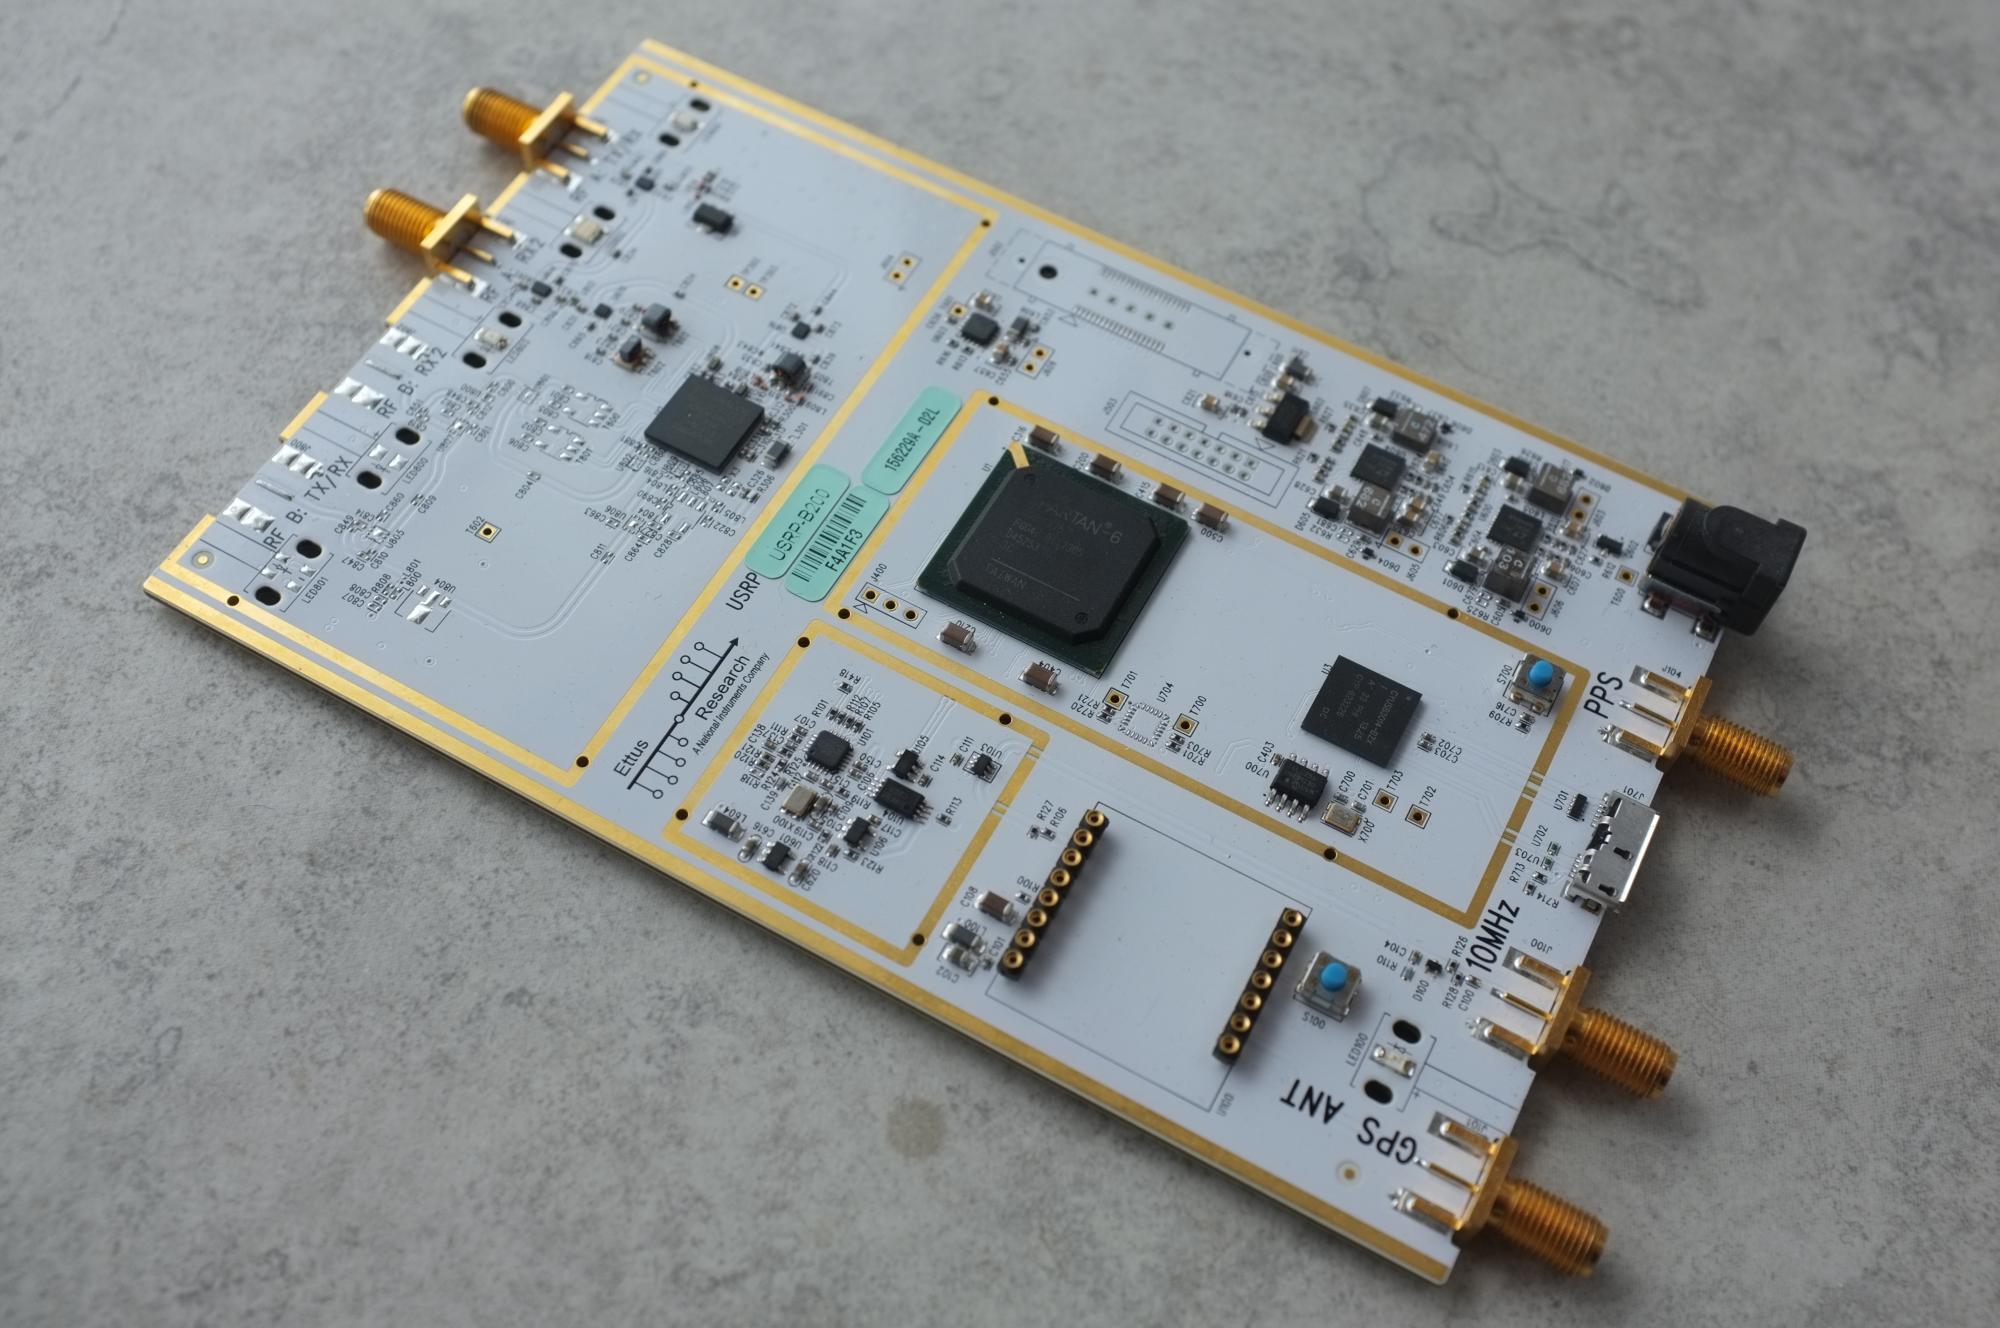
\includegraphics[width=12em]{figures/USRP-B200.jpg}
    \caption{Ettus USRP B200}
    \label{fig:usrp-b200}
\end{wrapfigure}


However, care has to be taken about the host system, especially about the USB
controller. Using USB~2.0 is not a problem for a DAB transmission, both USB~2.0
and USB~3.0 host controllers can therefore be used. Since USB~2.0 has been
around for longer and is more mature, it is sometimes preferable because it
causes less USB errors. This heavily depends on the exact model of the USB
controller inside the host PC, and has to be tested for each system.

The txgain on the B200 varies between $0$dB and about $90$dB. Experience shows
that compression effects begin to appear at values around $85$dB. This might be
different from device to device and needs to measured.

Similarly, the digital gain has to optimised for a given setting. It is
important that there is no digital clipping in the chain, because that leads to
problematic spurious spectrum components, that can disturb or even damage a
power amplifier.

There are some performance measurements available on the Opendigitalradio
wiki.\footnote{\url{http://wiki.opendigitalradio.org/index.php/USRP\_B200\_Measurements}}

\paragraph{Remarks concerning other USRP models}
We have used the USRP1, the USRP2 and the USRP B100 with the tools. The WBX is
the most appropriate daughterboard for these models.

The txgain setting has another range, it is best to start at $0$dB, and increase
it in steps of $3$dB or smaller while measuring the output signal, until the
correct power is reached.

\subsubsection{Other Hardware}
ODR-DabMod supports other radio interfaces using either standard output, or via
a fifo -- the latter must be created prior to runtime with the \texttt{mkfifo} command.
Due to limitations in the UHD driver library, \texttt{/dev/stdout} will only
function correctly if ODR-DabMod is configured at compilation time with the
following argument:

\begin{lstlisting}
--disable-output-uhd
\end{lstlisting}

ODR-DabMod has been tested working with HackRF from Great Scott Gadgets on i386 and
x86 architectures.\footnote{HackRF has not been tested to any degree of success
with ARM-based computers at this time as they are not (yet) capable of resampling
to the required higher rates as the process is highly CPU intensive.}

The unit is an entry level yet versatile SDR which provides coverage between
$\approx10$MHz to $6$GHz, and DAB signals been successfully generated with it in
VHF Band III ($174$--$240$MHz), L-Band ($1462$--$1467.5$MHz) and even the worldwide ISM
Band ($2400$--$2500$MHz). The latter (subject to local regulations) is a licence exempt
band which may be useful for performing freely radiating tests at low power. Cheap
MMDS converters are currently available which helpfully provide a Band III IF output
providing a direct feed to the aerial input of a receiver. Before choosing a converter
it is important to pay close attention to the specifications. The local oscillator
phase noise performance, and the dynamic range (due to the heavy use of the band) are
both particularly important.

To use HackRF, the output of ODR-DabMod must be set (in the configuration file) to
produce 8-bit signed integers, rather than the default complex floats.
HackRF has selectable baseband filters, however the lowest filter setting
($1.75$MHz) does not provide adequate image rejection at the native sampling rate of
$2048$k samples per second. An appropriate rate to start with is $4096$k, and for
some purposes this may well be adequate as this moves the image signals
generated within the radio far enough into the stop-band of filter to attenuate
them significantly. The digital gain in the ODR-DabMod configuration file should
be set to a maximum of $2.4$ at this rate to avoid digital clipping on modulation
peaks.

Example of the settings in the \texttt{mod.ini} file suitable for use with HackRF:

\begin{lstlisting}
[remotecontrol]
telnet=1
telnetport=2121

[input]
transport=file
source=myfirst.eti
loop=1

[modulator]
gainmode=2
digital_gain=2.4
rate=4096000

[firfilter]
enabled=1
filtertapsfile=filtertaps.txt

[output]
output=file

[fileoutput]
format=s8
filename=/tmp/ofdm.fifo

\end{lstlisting}

The output fifo has to be created beforehand, and the \texttt{hackrf\_transfer}
utility is then used to transmit the signal to the device.

Depending on the capabilities of the host computer, using higher sampling rates
($6144$k, and even $8192$k) may be possible. This oversampling is desirable as
it helps to produce a cleaner spectral output. At higher rates one needs to
ensure that samples are not being dropped on the USB and that CPU resources are
not being contended. It is also important to note that the digital gain value
must also be scaled accordingly as the sampling rate is increased. Two sets of
values are provided which reflect the theoretical values, and the second set
given in parentheses are empirical maximum values determined while monitoring
shoulder performance (measured at $970$kHz offset from the centre frequency)
using a spectrum analyser in $\approx 3$ kHz resolution bandwidth. The digital
gain figures for the tested sampling rates are shown below:

\begin{center}
\begin{tabular}{| l | c | c |}
    \hline
    Rate       & Dgain & Max Dgain (Empirical) \\ \hline \hline
    $4096$ksps & $2.0$ & $2.25$ \\ \hline
    $6144$ksps & $3.0$ & $3.37$ \\ \hline
    $8192$ksps & $4.0$ & $4.50$ \\
    \hline
\end{tabular}
\end{center}

The shoulder performance has been measured with shoulder performance at a little
better than $35$dB, which is roughly equivalent to that obtained from first
generation commercial modulator equipment. This can be increased to a relatively
respectable $\approx 40$dB by enabling the FIR baseband filter in ODR-DabMod,
and supplying it with an appropriate coefficient (tap) file. The maximum output
power available to mmet these performance figures is approximately $-10$dBm RMS.

Example of using ODR-DabMod with the \texttt{hackrf\_transfer} utility:

\begin{lstlisting}
mkfifo /tmp/ofdm.fifo
odr-dabmod mod.ini &
hackrf_transfer -t /tmp/ofdm.fifo -f 216928000 -x 47 \
    -a 1 -s 4096000 -b 1750000
\end{lstlisting}



\subsection{Audio Sources}
Preparing a DAB multiplex with different programmes requires that we are able to
read and encode several audio sources. We have seen in
section~\ref{sec:between_encoder_and_multiplexer} how the encoders can be
interfaced to the modulator. In this section we'll go through the different ways
to carry the audio data to the encoder.

\subsubsection{Local Audio Card}
It is possible to use an audio card connected to the computer as source. For
very simple scenarios, the ALSA input for FDK-AAC-DABplus is easiest to set up.
This however limits the usage of a single encoder per sound-card, and will not
scale well if more than one programme has to be encoded on the machine. It is
however ideal for dedicated encoding machines that can contribute the encoded
audio over an IP network.

An alternative to using ALSA is JACK\footnote{The JACK Audio Connection Kit is a
    virtual audio patch, \url{http://www.jack-audio.org}}
that can be used with a multi-channel sound card. JACK will expose every audio
input channel, and several encoders can be launched that also connect to JACK.
The input channels can be freely connected to the encoders thanks to the virtual
JACK patch panel.

\sidenote{It might be possible to use the libVLC input too, to be defined.}
FDK-AAC-DABplus supports JACK and ALSA input, but Toolame-dab supports only the
JACK input.

\subsubsection{Using Existing Web-Streams}
\label{usingexistingwebstreams}
One common scenario is to transmit radio stations that already are available as
web-radio streams. For simplicity, it makes sense to get these web streams,
which are most often encoded in mp3 and available through HTTP, decode them, and
use them as audio source for the DAB or \dabplus encoder.

The advantage of this approach is that the radio itself does not need to setup a
new infrastructure if the stream is of good quality. The main disadvantage is
that the audio is encoded twice, and this coding cascading degrades the audio
quality.

Often, web-streams are encoded in mp3 at $44100\Hz$ sample-rate, whereas DAB
is most often $48000\Hz$ or sometimes $32000\Hz$. A sample-rate conversion is
necessary in the stream decoder.

There are many different stream decoders, and gstreamer, mpg123 and mplayer have
been tested. By far the easiest way is to use the libVLC binding that can be
compiled for Toolame-dab and FDK-AAC-DABplus. This library has
the same features as the VLC audio player, but the audio data is directly passed
to the encoding routines. This allows the encoder to receive all network
sources VLC supports, not only HTTP web-streams but also less common setups
e.g.\ encoded audio inside multicast UDP MPEG-TS.
This is illustrated in ``Studio A'' in figure~\ref{fig:txchain-with-encoders}.

We have also achieved good results with mplayer, and the dab-scripts
repository\footnote{\url{http://github.com/Opendigitalradio/dab-scripts}}
contains the script \texttt{encode-jack.sh} that uses mplayer, and illustrates
how it is possible to encode a web-stream to \dabplus. JACK is used to
interconnect the stream decoder to the \dabplus encoder.
This is illustrated in ``Studio B''.

\begin{figure}[h]
    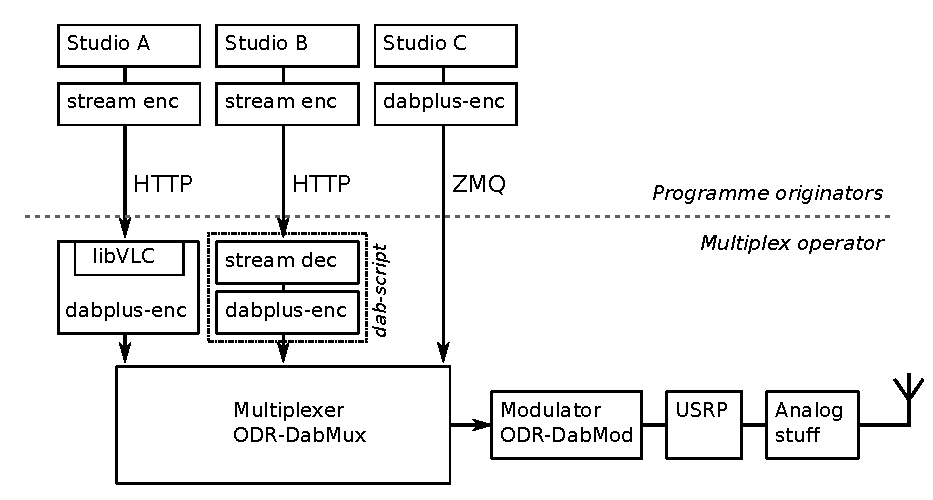
\includegraphics[width=\textwidth]{figures/txchain-with-encoders.pdf}
    \caption{Three common ways to encode a remote audio sources.}
    \label{fig:txchain-with-encoders}
\end{figure}


The scripts are designed for production use, and also contain automatic restart
logic in case of a failure. They send an email and write a message into the
system log.

\subsubsection{Encoders at Programme Originator Studios}
In order to avoid the unavoidable encoder cascading when using mp3 web-streams,
the DAB or \dabplus encoder has to be moved to the programme originator's
premises, and should directly encode the audio signal coming from the studios.
This is illustrated in ``Studio C'' in figure~\ref{fig:txchain-with-encoders}.


\subsection{Single-Frequency Networks}
